\chapter{Исследовательская часть}
В исследовательской части проводится изучение производительности системы визуализации трёхмерного огня.

\section{Методика исследования производительности}

Целью исследования является анализ влияния количества частиц на производительность системы визуализации. Исследование включает изучение зависимости частоты кадров от общего количества частиц, влияние внешнего освещения, а также наличие алгоритма z-буфера.

Параметры исследования:
\begin{enumerate}
	\item количество частиц в сцене: от 10 000 до 2 000 000;
	\item наличие внешнего освещения;
	\item использование алгоритма z-буфера.
\end{enumerate}

Изменение производительности вычисляется по формуле:

\[
\Delta P = \left(1 - \frac{\text{FPS}_{\text{результат1}}}{\text{FPS}_{\text{результат2}}}\right) \times 100\%,
\]

Измерения проводились на системе с процессором Intel Core i9-14900K (24 ядра, 8 логических ядер)~\cite{IntelSDM}, видеокартой NVIDIA GeForce RTX 4090 и 64 ГБ оперативной памяти. Все тесты выполнялись при разрешении 800×600 пикселей.

\section{Анализ производительности системы}

\subsection{Зависимость частоты кадров от количества частиц}

На рисунке \ref{fig:graph-particles} и в таблице \ref{tab:fps-particles} представлена зависимость частоты кадров от количества частиц.

\begin{figure}[h!]
	\centering
	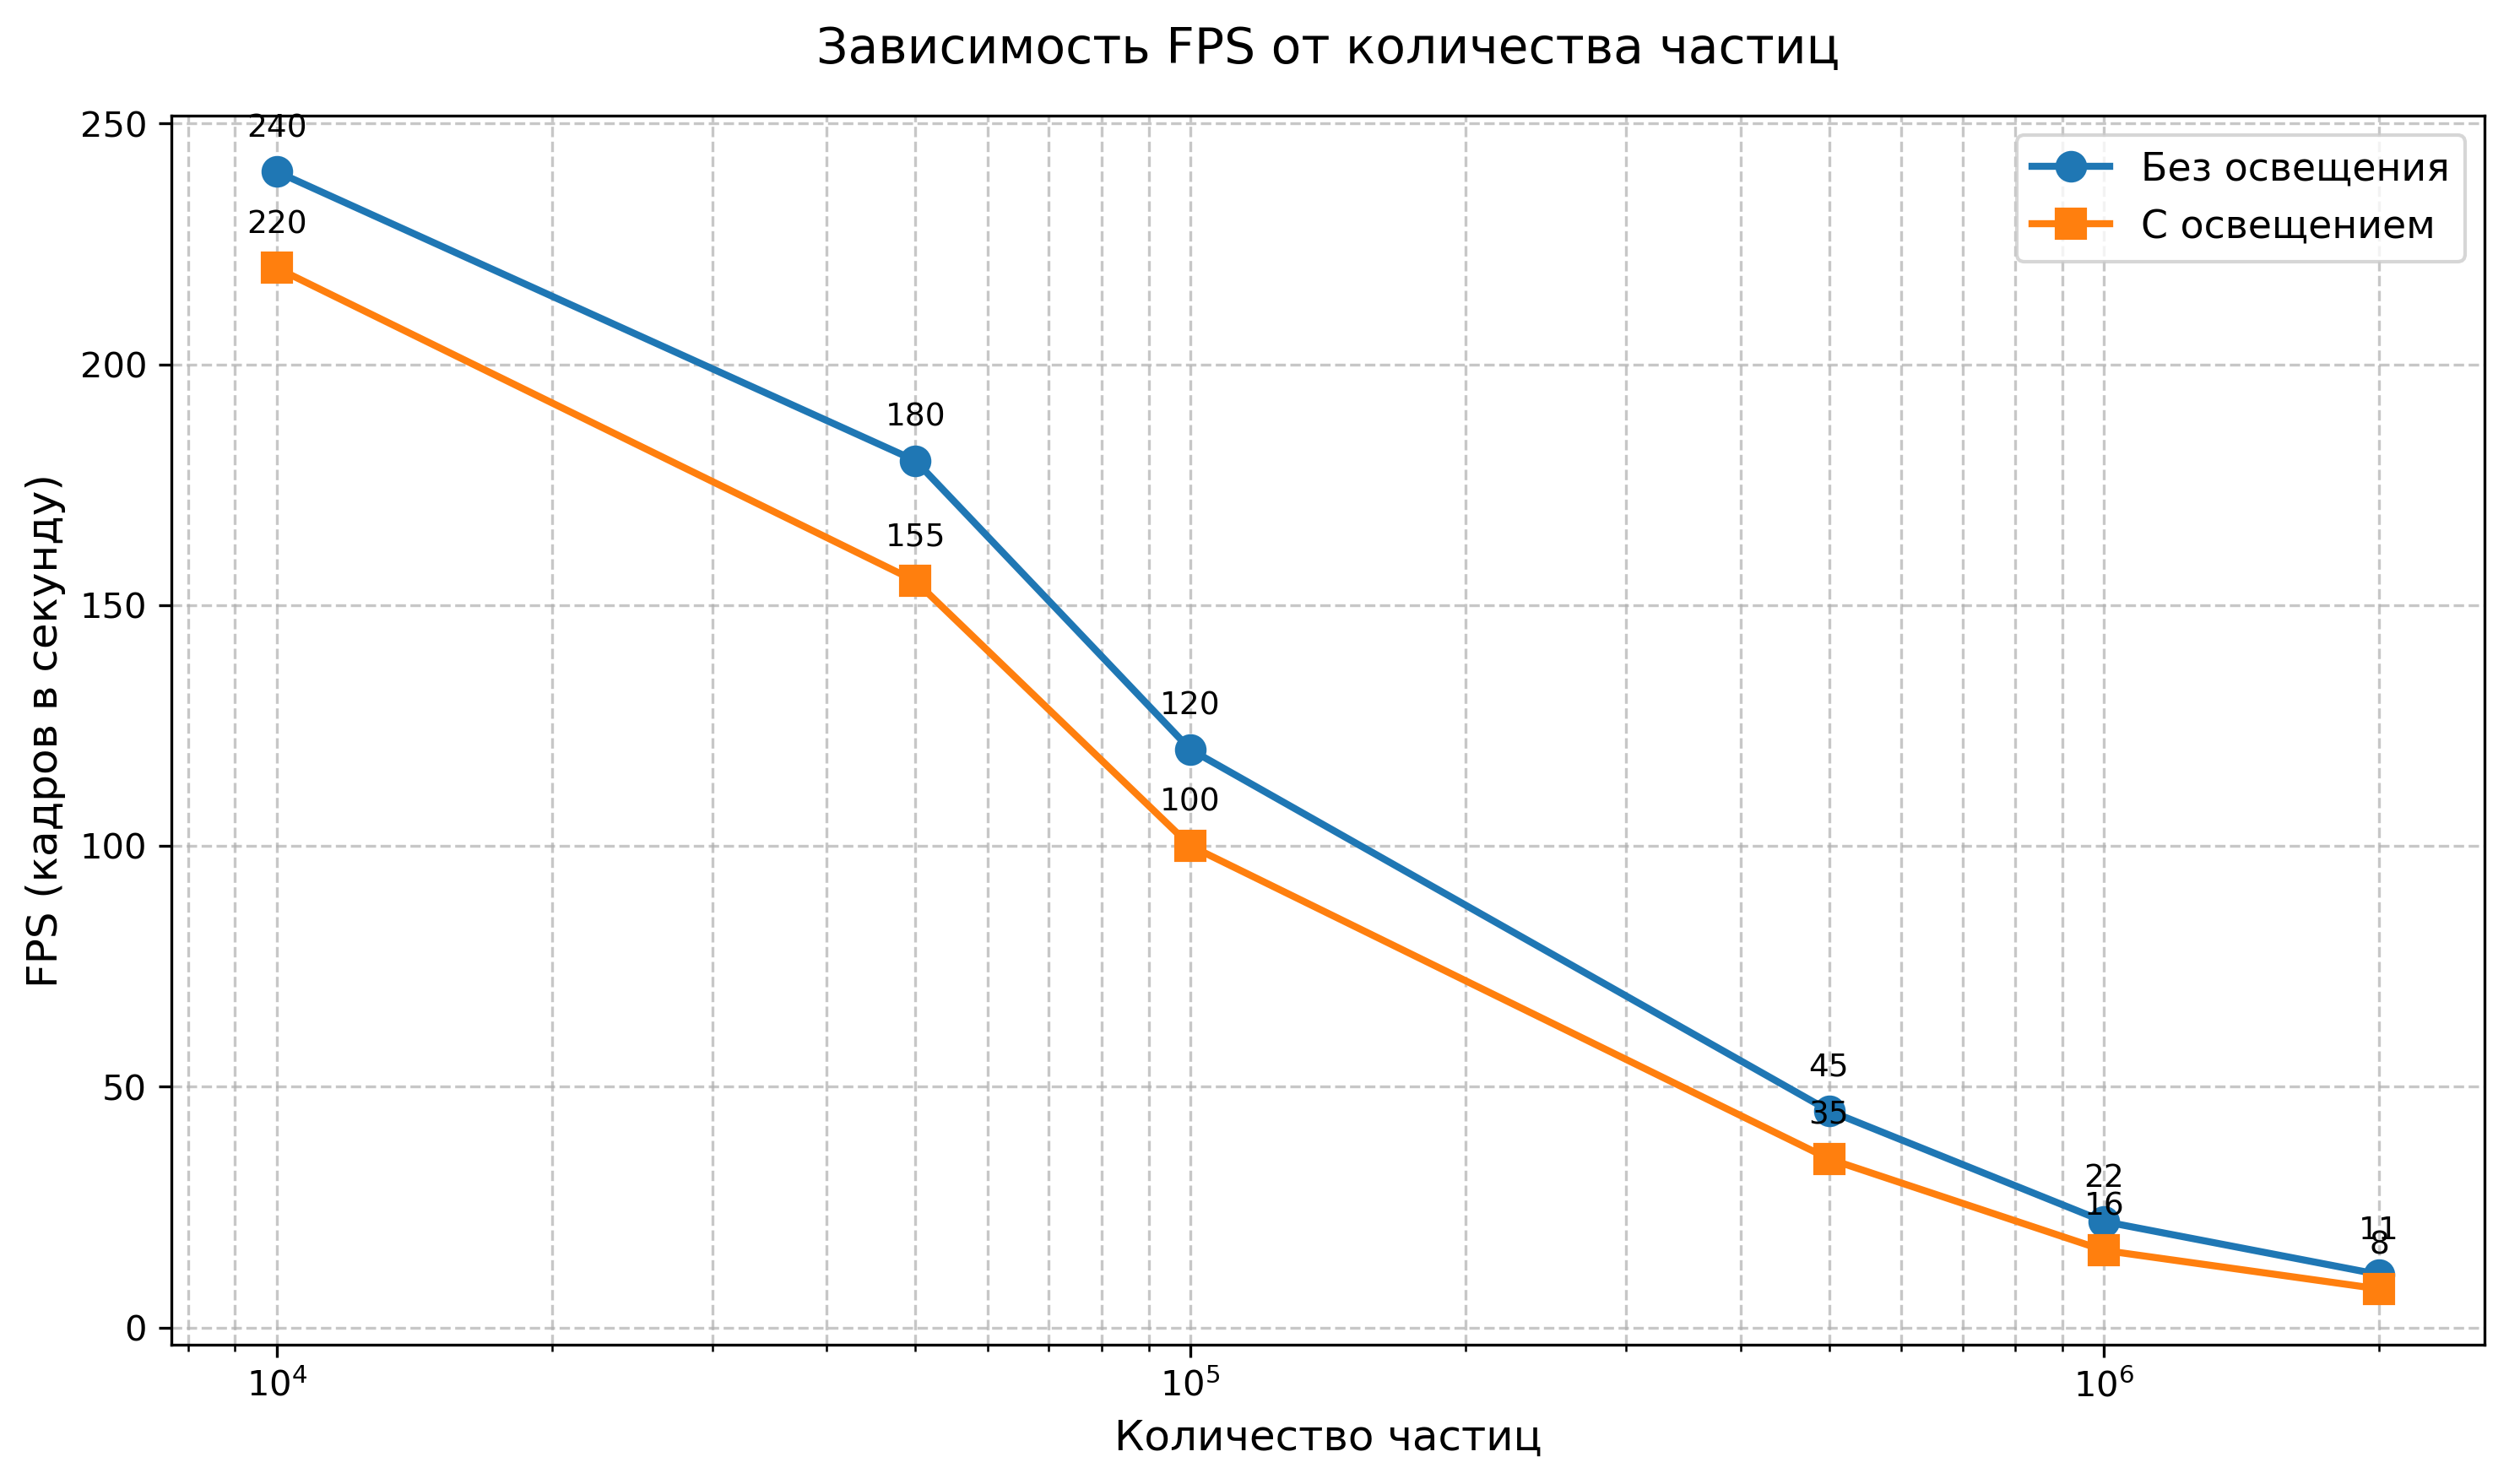
\includegraphics[width=0.85\textwidth]{graph_particles.png}
	\caption{График зависимости частоты кадров от количества частиц}
	\label{fig:graph-particles}
\end{figure}


\begin{table}[h!]
	\centering
	\caption{Зависимость частоты кадров от количества частиц}
	\label{tab:fps-particles}
	\begin{tabular}{|c|c|c|c|}
		\hline
		\textbf{Количество частиц} & \textbf{FPS (без освещения)} & \textbf{FPS (с освещением)} & \textbf{Снижение, \%} \\ \hline
		10 000  & 240 & 220 & 8.3 \\ \hline
		50 000  & 180 & 155 & 13.9 \\ \hline
		100 000 & 120 & 100 & 16.7 \\ \hline
		500 000 & 45  & 35  & 22.2 \\ \hline
		1 000 000 & 22 & 16 & 27.3 \\ \hline
		2 000 000 & 11 & 8  & 27.3 \\ \hline
	\end{tabular}
\end{table}

С увеличением количества частиц частота кадров закономерно снижается. При использовании внешнего освещения наблюдается дополнительное снижение производительности. Увеличение количества частиц с 10 000 до 2 000 000 приводит к снижению частоты кадров более чем в 20 раз. Включение внешнего освещения дополнительно снижает производительность на 8–27\%.

	\subsection{Зависимость от наличия z-буфера}

Для оценки влияния алгоритма z-буфера проведено сравнение производительности при его использовании и без него. Результаты представлены в таблице \ref{tab:z-buffer} и на рисунке \ref{fig:z-buffer-graph}.

\begin{table}[h!]
	\centering
	\caption{Сравнение производительности с использованием z-буфера и без него (100 000 частиц)}
	\label{tab:z-buffer}
	\begin{tabular}{|c|c|c|c|}
		\hline
		\textbf{Режим рендеринга} & \textbf{FPS (без освещения)} & \textbf{FPS (с освещением)} & \textbf{Затраты, \%} \\ \hline
		С использованием z-буфера & 120 & 100 & -- \\ \hline
		Без использования z-буфера & 160 & 135 & 25.0–35.0 \\ \hline
	\end{tabular}
\end{table}

\begin{figure}[h!]
	\centering
	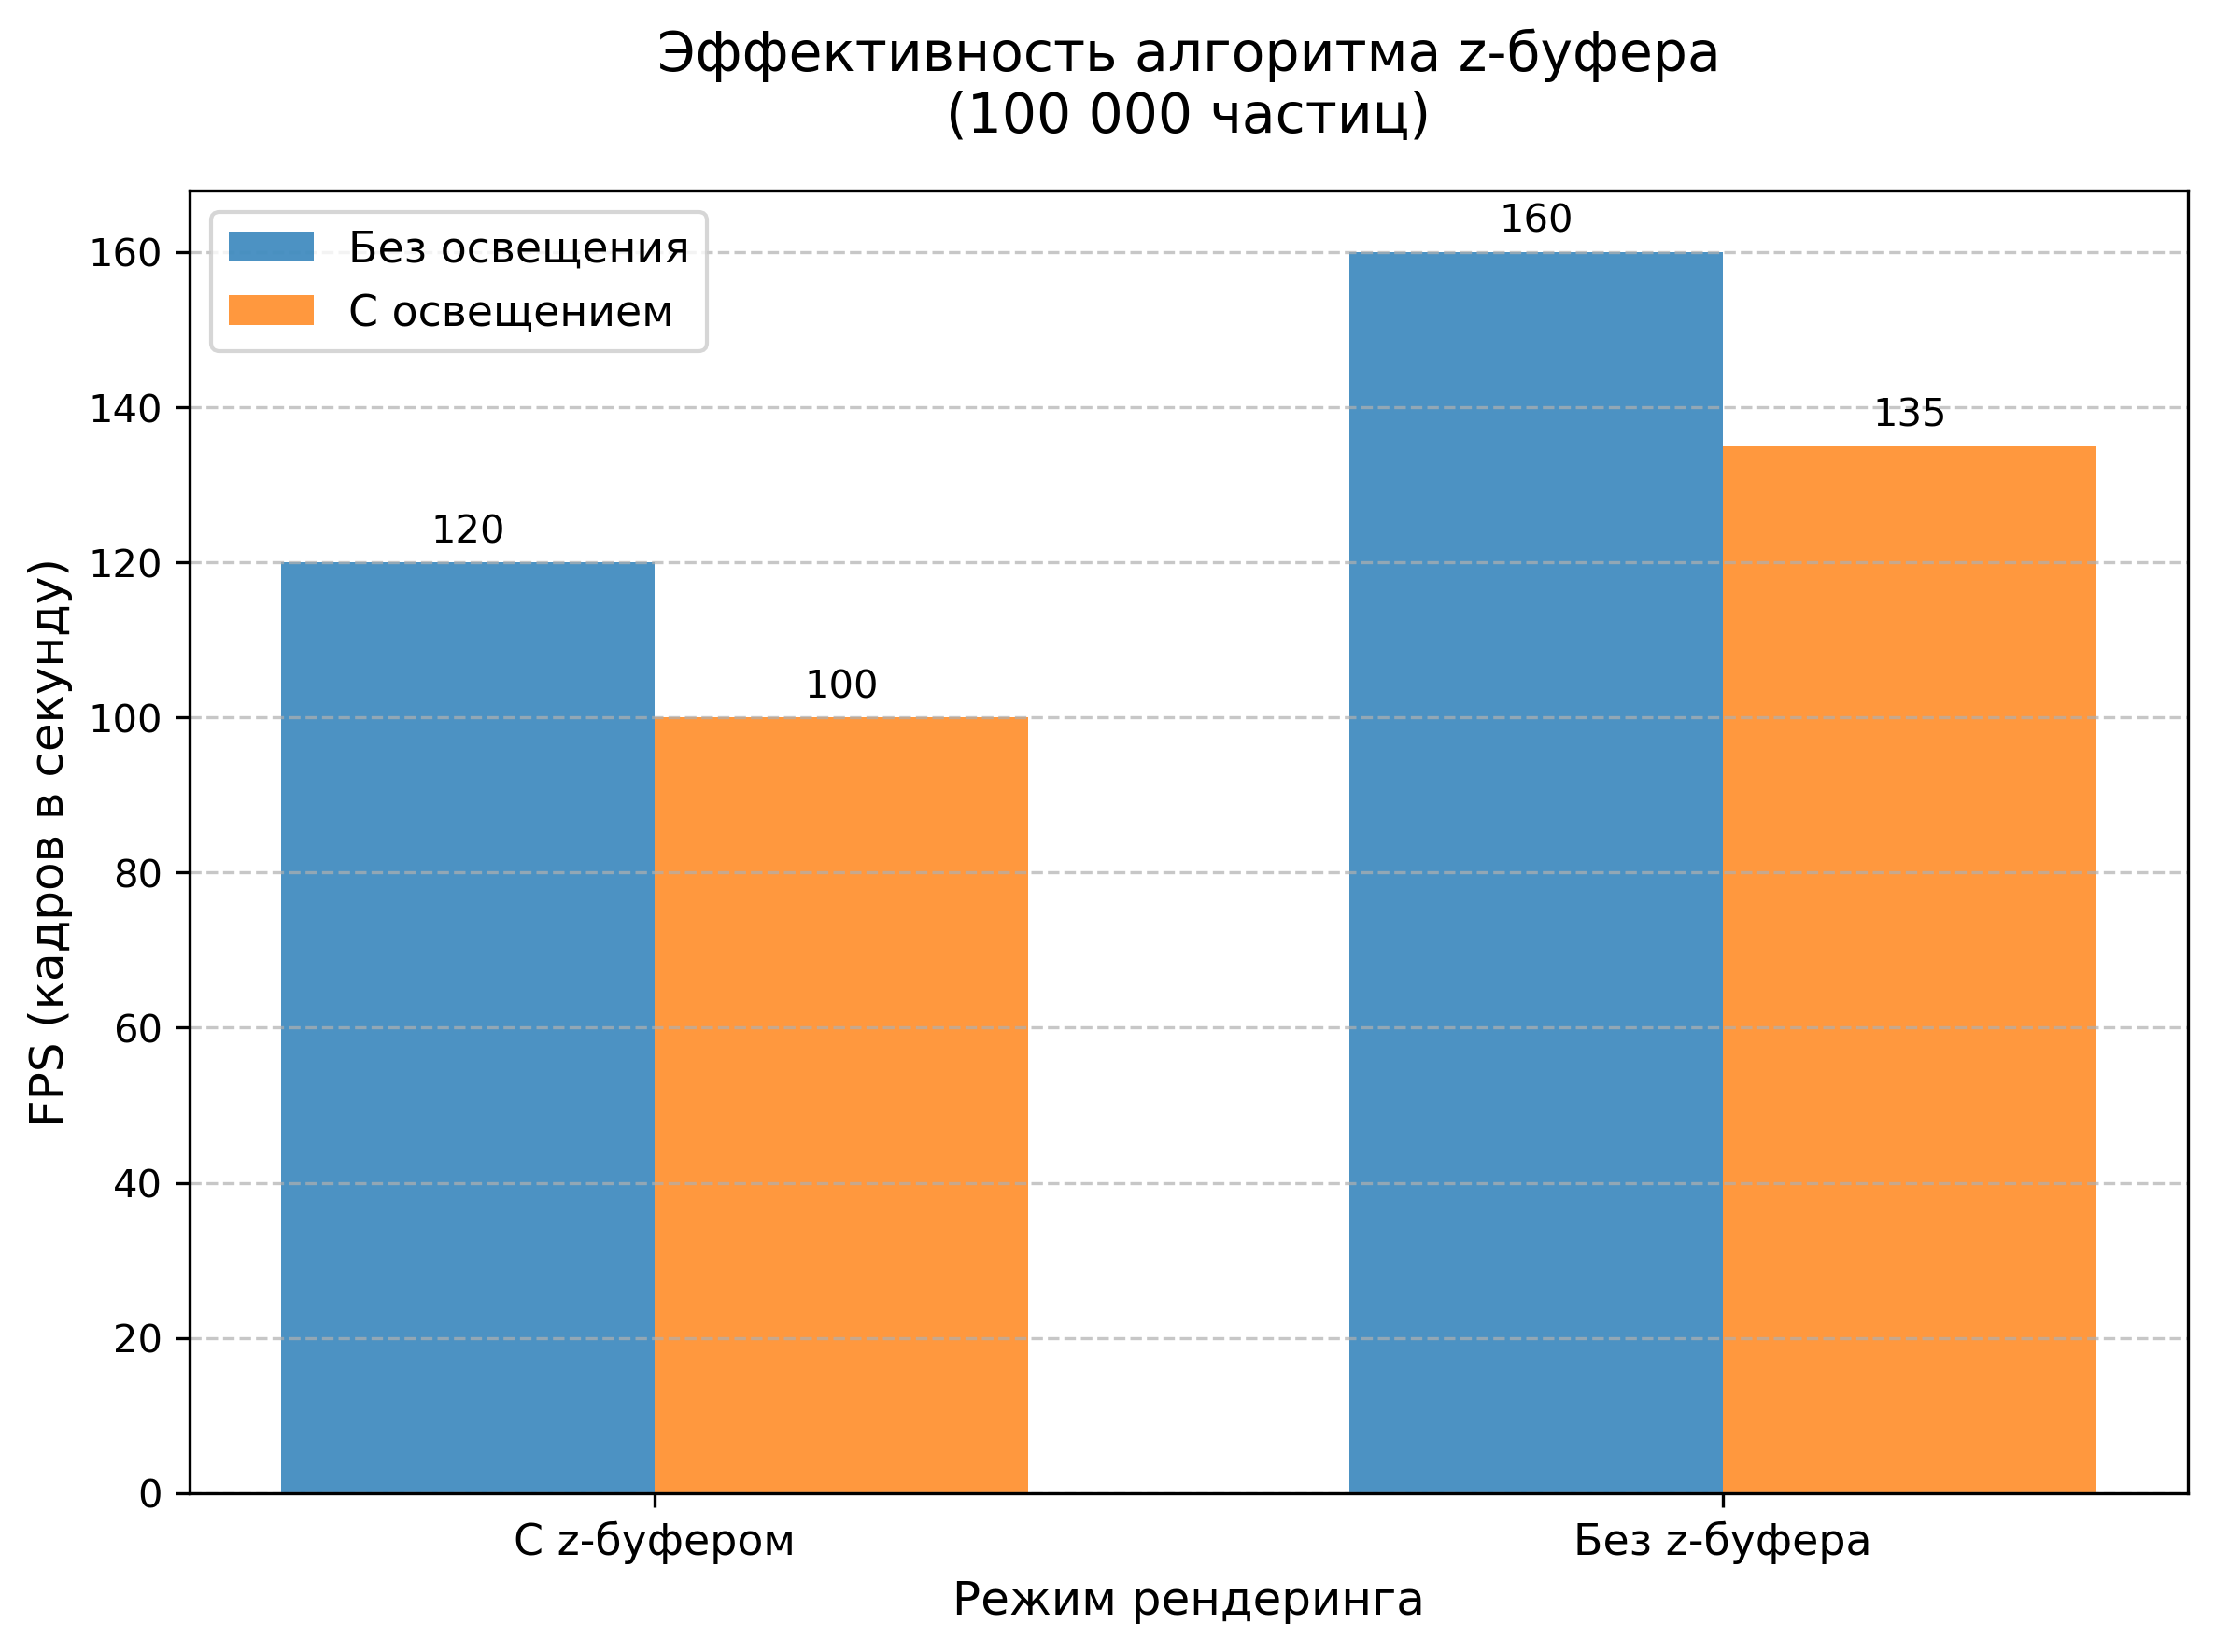
\includegraphics[width=0.6\textwidth]{graph_z_buffer.png}
	\caption{График сравнения производительности с использованием z-буфера и без него}
	\label{fig:z-buffer-graph}
\end{figure}

Аалгоритм z-буфера обеспечивает корректное отображение частиц по глубине, но вносит дополнительные вычислительные затраты в размере 25–35\% по сравнению с рендерингом без проверки глубины. При отключении z-буфера производительность возрастает, однако нарушается визуализация: частицы, находящиеся дальше от камеры, могут отображаться поверх более близких.

\section{Вывод}

В рамках исследовательской части проведено изучение производительности системы визуализации трёхмерного огня: проанализировано влияние количества частиц на частоту обновления кадров, исследована эффективность алгоритма z-буфера и оценено влияние внешнего освещения на производительность.

\clearpage